\documentclass[11pt,a4paper]{extarticle}
\usepackage[utf8]{inputenc}
\usepackage{amsmath}
\usepackage{amsfonts}
\usepackage{amssymb}
\usepackage{graphicx}
\usepackage{natbib}
\usepackage[utf8]{inputenc}
\usepackage{tikz}
\usetikzlibrary{arrows}
\usepackage{hyperref}
\usepackage{verbatim}
\usepackage{array}
\usepackage{subcaption}
\usepackage{tablefootnote}
\usepackage{listings}
\usepackage{enumitem}
\usepackage[a4paper]{geometry}
%\newgeometry{left=3cm,bottom=3cm, right=3cm, top=3cm}

\author{Joren Verspeelt, Jochem Geussens, Vincent Tanghe}
\title{Semantic Embeddings in IR \\
	\large Text-Based Information Retrieval}

\DeclareGraphicsExtensions{.pdf,.png,.jpg}
\renewcommand{\figurename}{Fig.}
\renewcommand{\refname}{}
\newcolumntype{L}{>{\centering\arraybackslash}m{3cm}}
\newcolumntype{C}[1]{>{\centering\let\newline\\\arraybackslash\hspace{0pt}}m{#1}}


\newcommand{\myitembf}[2] {
	\item \textbf{#1 :} #2
}
\newcommand{\myitem}[2] {
	\item #1 : #2
}
\newcommand{\tab}{
	\-\quad
}

\newcommand{\mypageref}[1] {
	[page \pageref{#1}]
}

\begin{document}
\maketitle

\section {Introduction}
In the field of Natural Language Processing (NLP) and Information Retrieval (IR), there is a large need for good presentations of text documents. Recently, a lot of researchers in the field are presenting dense word representations (also known as Word Embeddings, Neural Embeddings or Sementic Embeddings).
For the Course of Text-Based Information Retrieval, we are given the opportunity to work with state-of-the-art algorithms. The goal of this assignment is to gain practical experience with these algorithms by comparing them and using them in an application. 
First we will implement a small analogy solver that guesses related words given a simple analogy. Then, we will discuss our implementation for a search engine to find pictures based on their description.


\clearpage
\tableofcontents
\clearpage



\section {Part I (Warm-up)}
\subsection{Task description}
In this part, we discuss two analogy solvers that try to guess the correct word, given simple analogy questions. E.g.:

\begin{align*}
	a : b = c : ?\\
	Bratislava : Slovakia = Bishkek : ?\\
	ate : eat = found : ?
\end{align*}
\newline
Then, we will run several analogy solving models with several different representations on the benchmarking analogy dataset.


\subsection{Setup}
We compare the use of different word embeddings (GloVe and Word2Vec) towards different analogy arithmetic models\cite{marekreiblog}. To test these, we used the questions provided by Google\cite{word2vecquestionwords}.
\newline
\newline
We coded our solution in Python (version 2.7) using Jupyter Notebook. All experiments were run on a notebook with 8GB RAM memory, Intel(R) CORE\textsuperscript{TM}i7-3610QM CPU, SSD hard disk and a Windows 7 Operating System.
\newline
\newline
We use freely available pretrained vector models for GloVe \cite{glovedata} and Word2Ve \cite{word2vecdata}. The GloVe models are almost the same format as the Word2Vec models, the only difference is that Word2Vec had a header with the dimensions. Once these headers are added, the GloVe model can also run with the default Gensim operations for Word2Vec.
\newline
\newline
To run the different analogy arithmetic models (see next paragraph), we introduce a separate function in our code for each model. These functions then use the Gensim library for Python \cite{gensim} to calculate the different vector distances.
\newline
\newline
\textbf{An analogy arithmetic function} is used to calculate how close the input vector is to another vector in order to choose the most similar result. To calculate the angle between high dimensional vectors, Mikolov et al. \cite{mikolov} proposed using cosine similarity as explained in equation \ref{cosinesimilarity}. 
\begin{equation}
\begin{split}
\label{cosinesimilarity}
similarity(v1, v2) &= cos(\theta) \\&= \dfrac{v1 \cdot v2}{||v1|| \cdot ||v2||}  \\&= \dfrac{\sum_{i=1}^{n}v1_i v2_i}{\sqrt{\sum_{i=1}^{n}v1_i^2} \sqrt{\sum_{i=1}^{n} v2_i^2}}
\end{split}
\end{equation}

\leavevmode
\newline
We consider two analogy arithmetic models. The first is named the \textbf{Addition method} and is simply maximizing the cosine similarity between the result $d_w$ and the vector equation $c-a+b$, where the variables $a, b and c$ have the same meaning as mentioned in the warm-up exercise. This method actually looks for words similar to c and b, and not to a. In equation \ref{additionmethod} we introduce $V$ as the whole vocabulary and $d'_w$ as a chosen element from $V$.

\begin{equation}
\begin{split}
\label{multiplicationmethod}
v &= c-a+b\\
d_w &= argmax_{d'_w \in V}(similarity(d'_w, v) )
\end{split}
\end{equation}
\newline
The other method was referred to as the \textbf{Multiplication method} \cite{leviandgoldberg}. Because the Addition method risks being dominated by one large term, therefore the authors proposed that instead of adding the similarities, they could be multiplied as described in equation \ref{multiplicationmethod}.

\begin{equation}
\begin{split}
\label{multiplicationmethod}
d_w &= argmax_{d'_w \in V}(\dfrac{similarity(d'_w, c) similarity(d'_w, b)}{similarity(d'_w, a) + \epsilon} )
\end{split}
\end{equation}
\newline
\textbf{Two different recall numbers} are generated if a word does not occur within the pretrained vector model: One where the \textbf{missing word is considered a failure} for the analogy and one where the \textbf{missing word is just ignored}. We could also have done a third option, were we use the nearest word in the vector model instead of the missing word. However, we did not do this because this would take a lot more computing power and (as seen in the results below) we're not sure whether it would have made a difference.

\subsection{Results}
\label{sec:tabellen}
\begin{table}[h!]
\centering
\begin{tabular}{|c|c|}
   	\hline
   	\textbf{Category} &    \textbf{Recall}\\ \hline
   	Capital common countries 	& 0.83202 \\
   	Capital World 				& 0.79134 \\
   	Currency					& 0.35104 \\
   	City in state				& 0.70896 \\
   	Family 						& 0.84585 \\
   	Gram1 adjective to adverb 	& 0.28528 \\
   	Gram2 opposite 				& 0.42734 \\
   	Gram3 comparative 			& 0.90841 \\
   	Gram4 superlative 			& 0.87344 \\
   	Gram5 present participle	& 0.78125 \\
   	Gram6 nationality adjective & 0.89931 \\
   	Gram7 past tense 			& 0.65962 \\
   	Gram8 plural 				& 0.89865 \\
   	Gram9 plural verbs 			& 0.67931 \\
   	\textbf{Total}				& 0.73588 \\ \hline
\end{tabular}
\caption{Word2Vec addition model (ran for 1h15)}
\label{table:word2vec_addition}
\end{table}

\begin{table}[h!]
\centering
\begin{tabular}{| l | c | r}
   	\hline
   	\textbf{Category} &    \textbf{Recall}\\ \hline
   	Capital common countries 	& 0.85178 \\
   	Capital World 				& 0.80570 \\
   	Currency					& 0.35450 \\
   	City in state				& 0.71423 \\
   	Family 						& 0.84585 \\
   	Gram1 adjective to adverb 	& 0.31552 \\
   	Gram2 opposite 				& 0.42365 \\
   	Gram3 comparative 			& 0.90691 \\
   	Gram4 superlative 			& 0.91800 \\
   	Gram5 present participle	& 0.80587 \\
   	Gram6 nationality adjective & 0.89368 \\
   	Gram7 past tense 			& 0.70641 \\
   	Gram8 plural 				& 0.89940 \\
   	Gram9 plural verbs 			& 0.73448 \\
   	\textbf{Total}				& 0.75148 \\ \hline
\end{tabular}
\caption{Word2Vec multiplication model (ran for 3h25)}
\label{table:word2vec_multiplication}
\end{table}

GloVe always had the same amount of skipped words (all words) independent of the dimension within a category. So we will not show the category results for these.

\begin{table}[h!]
	\centering
\begin{tabular}{| l | c | r}
    	\hline
    	\textbf{Category} &    \textbf{Recall}\\ \hline
    	Family 						& 0.85573 \\
    	Gram1 adjective to adverb 	& 0.25403 \\
    	Gram2 opposite 				& 0.22660 \\
    	Gram3 comparative 			& 0.86486 \\
    	Gram4 superlative 			& 0.69786 \\
    	Gram5 present participle	& 0.68277 \\
    	Gram7 past tense 			& 0.60192 \\
    	Gram8 plural 				& 0.77402 \\
    	Gram9 plural verbs 			& 0.59770 \\
    	\textbf{Total}				& 0.30778 \\
    	\textbf{Total no skipped}	& 0.62774 \\ \hline
\end{tabular}
\caption{GloVe50d addition model (ran for 3 min)}
\label{table:glove50d_addition}
\end{table}

\begin{table}[h!]
	\centering
\begin{tabular}{| l | c | r}
    	\hline
    	\textbf{Category} &    \textbf{Recall}\\ \hline
    	Family 						& 0.62846 \\
    	Gram1 adjective to adverb 	& 0.09980 \\
    	Gram2 opposite 				& 0.04926 \\
    	Gram3 comparative 			& 0.41366 \\
    	Gram4 superlative 			& 0.17112 \\
    	Gram5 present participle	& 0.29451 \\
    	Gram7 past tense 			& 0.31153 \\
    	Gram8 plural 				& 0.46021 \\
    	Gram9 plural verbs 			& 0.25862 \\
    	\textbf{Total}				& 0.14506 \\
    	\textbf{Total no skipped}	& 0.29587 \\ \hline
\end{tabular}
\caption{GloVe50d multiplication model (ran for 3 min)}
\label{table:glove50d_addition}
\end{table}


\begin{table}[h!]
	\centering
\begin{tabular}{| l | c | r}
    	\hline
    	\textbf{Category} &    \textbf{Recall}\\ \hline
    	Family 						& 0.81621 \\
    	Gram1 adjective to adverb 	& 0.24395 \\
    	Gram2 opposite 				& 0.20074 \\
    	Gram3 comparative 			& 0.79129 \\
    	Gram4 superlative 			& 0.54278 \\
    	Gram5 present participle	& 0.69508 \\
    	Gram7 past tense 			& 0.55448 \\
    	Gram8 plural 				& 0.71997 \\
    	Gram9 plural verbs 			& 0.58391 \\
    	\textbf{Total}				& 0.28382 \\
    	\textbf{Total no skipped}	& 0.57890 \\ \hline
\end{tabular}
\caption{GloVe100d addition model (ran for 7 min)}
\label{table:glove100d_addition}
\end{table}

\begin{table}[h!]
	\centering
\begin{tabular}{| l | c | r}
    	\hline
    	\textbf{Category} &    \textbf{Recall}\\ \hline
    	Family 						& 0.77866 \\
    	Gram1 adjective to adverb 	& 0.22883 \\
    	Gram2 opposite 				& 0.15764 \\
    	Gram3 comparative 			& 0.74850 \\
    	Gram4 superlative 			& 0.50624 \\
    	Gram5 present participle	& 0.65057 \\
    	Gram7 past tense 			& 0.52821 \\
    	Gram8 plural 				& 0.66667 \\
    	Gram9 plural verbs 			& 0.57356 \\
    	\textbf{Total}				& 0.26668 \\
    	\textbf{Total no skipped}	& 0.54394 \\ \hline
\end{tabular}
\caption{GloVe100d multiplication model (ran for 7 min)}
\label{table:glove100d_addition}
\end{table}



\begin{table}[h!]
	\centering
\begin{tabular}{| l | c | r}
    	\hline
    	\textbf{Category} &    \textbf{Recall}\\ \hline
    	Family 						& 0.85573 \\
    	Gram1 adjective to adverb 	& 0.25403 \\
    	Gram2 opposite 				& 0.22660 \\
    	Gram3 comparative 			& 0.86486 \\
    	Gram4 superlative 			& 0.69786 \\
    	Gram5 present participle	& 0.68277 \\
    	Gram7 past tense 			& 0.60192 \\
    	Gram8 plural 				& 0.77402 \\
    	Gram9 plural verbs 			& 0.59770 \\
    	\textbf{Total}				& 0.30778 \\
    	\textbf{Total no skipped}	& 0.62774 \\ \hline
\end{tabular}
\caption{GloVe200d addition model (ran for 10 min)}
\label{table:glove200d_addition}
\end{table}

\begin{table}[h!]
	\centering
\begin{tabular}{| l | c |}
    	\hline
    	\textbf{Category} &    \textbf{Recall}\\ \hline
    	Family 						& 0.85178 \\
    	Gram1 adjective to adverb 	& 0.25302 \\
    	Gram2 opposite 				& 0.19581 \\
    	Gram3 comparative 			& 0.83784 \\
    	Gram4 superlative 			& 0.67162 \\
    	Gram5 present participle	& 0.67045 \\
    	Gram7 past tense 			& 0.60321 \\
    	Gram8 plural 				& 0.76426 \\
    	Gram9 plural verbs 			& 0.65172 \\
    	\textbf{Total}				& 0.03531 \\
    	\textbf{Total no skipped}	& 0.62273 \\ \hline
\end{tabular}
\caption{GloVe200d multiplication model (ran for 10 min)}
\label{table:glove200d_multiplication}
\end{table}

\begin{table}[h!]
	\centering
\begin{tabular}{| l | c | r}
    	\hline
    	\textbf{Category} &    \textbf{Recall}\\ \hline
    	\textbf{Total}				& 0.31304 \\
    	\textbf{Total no skipped}	& 0.63849 \\ \hline
\end{tabular}
\caption{GloVe300d addition model (ran for 20 min)}
\label{table:glove300d_addition}
\end{table}

\begin{table}[h!]
	\centering
\begin{tabular}{| l | c |}
    	\hline
    	\textbf{Category} 			& \textbf{Recall}\\ \hline
    	\textbf{Total}	  			& 0.32214 \\
    	\textbf{Total no skipped}	& 0.65707 \\ \hline
\end{tabular}
\caption{GloVe300d multiplication model (ran for 20 min)}
\label{table:glove300d_multiplication}
\end{table}

\begin{figure}[ht!]
\centering
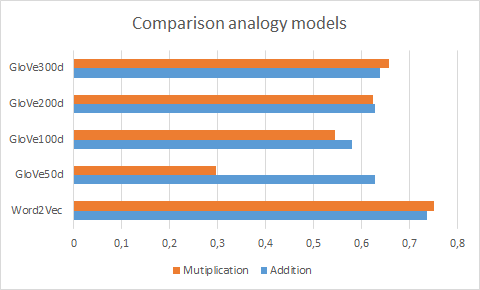
\includegraphics[width=130mm]{images/chart1.png}
\caption{}
\end{figure}


\subsection{Discussion}
We noticed that the GloVe model was not able to find all the words and this influences the results regarding execution times. The GloVe model seems to run a lot faster than the Word2Vec model because of our implementation strategy. If one word of the analogy is missing, the whole analogy is skipped resulting in smaller search space that needs to be covered. But that aside the GloVe model has the edge with faster calculations due to its lower dimensionality.
\newline
\newline
The complexity of the analogy models are O(3n) as 3 vectors need to be found in the space of n available vectors in our model. Worst case these vectors are at the end.
\newline
\newline
If we look at the dimensionality of the GloVe representations, we see that the overall accuracy increases as the number of dimensions increases. This is a trade-off compared to the time needed to run the model, but in general it seems worthwhile. 
If we then look at the analogy model compared to the dimensionality, we see that the multiplication model performs better on higher dimensions while the addition model performs better as the dimension decrease. The overall accuracy decrease with a lower dimension is most likely the reason for this.
\newline
\newline
While running the experiment, we frequently got missing words (using the GloVe representation). It is still impractical to have a model representing every possible word that exists, so a trade-off is made towards a reasonable model size and the amount of represented words. We solved this problem by either counting missing words as failed analogies or by skipping the sentence. However, it seems that the same word categories are missing in every dimension and counting only makes the accuracy worse.






\section{Part II}
\subsection{Task description}
This part of the assignment is based on the annual Scalable Concept Image Annotation Challenge, organized by ImageCLEF \cite{imageclef}. The dataset (given by ImageCLEF), contains sentence descriptions aligned to actual images. In this part of the assignment, we bring our previous tests into a real-life retrieval scenario: retrieve images by their descriptions using textual queries. Each query has a corresponding image ID, which can be used to verify the correctness of the model. The goal is to match queries with image descriptions as good as possible, using precision and recall as evaluation measures.
\newline
\newline
First we implemented a simple language model to retrieve the images, this was based on a unigram implementation \cite{languagemodelsforinformationretrieval}. Afterwards we extended it with word embedding, inspired by part I of this assignment. For the final method, we chose to implement Latent Dirichlet Allocation (LDA) with dirichlet priors. We have read that this performs well with twitter data, where the document size seems similar to our image descriptions. And this is a method that has been mentioned several times in class which sparked our interest. 


\subsection{Setup}
We coded our solution in Python (version 3+) using Jupyter Notebook and regular python files. All experiments were run on a notebook with 8GB RAM memory, Intel(R) CORE\textsuperscript{TM}i7-3610QM CPU, SSD hard disk and a Windows 7 Operating System.

\paragraph{The data}
we received contains the following documents:
\begin{description}
	\item[A. target\_collection] A table representing 17,784 images with as columns a unique numerical ID, an ID that corresponds to the actual image file and a description of the image. This data is used to train our model.
	\item[B. queries\_val] A similar table as the \textit{target\_collection} but it represents 1000 different images. This table will be used to test the accuracy of our trained model.
	\item[B. test queries\_val] A collection similar to \textit{queries\_val} but it only contains 200 queries and it does not tell which image id should be returned. This file is the real test data where we can't tune our method for optimal results. The similarities will be used to rate our results to other students.
\end{description}

\paragraph{Preprosessing}
Because comparison of words happen on the exact format of the words, we decided to do some preprocessing to make sure every word is in the same base form. Both the target collection as the queries were lemmatized. And, because we find that some words carry more meaning than other words, we also decided to remove the punctuation using regular expressions and the stop words (e.g. the, it, to, ...) using the freely available stop words list 2 (stopwordlist2 - http://www.lextek.com/manuals/onix/stopwords2.html).
\newline
\newline
Furthermore, we noticed that all queries and the target data are written in British English. Because we use the pre-trained Google News vector model, which only contains American English words, a lot of remained not found. So we did a hardcoded translation of the most frequent missing words - due to the lack of a good library - for the embedding results.
\newline
\newline
We will report the Recall and \textit{Mean Average Precision} (MAP) with a cutoff of 1000 documents in our results.

\subsection{Results}
\subsubsection{Unigram Language Model}
\begin{figure}[H]
	\centering
	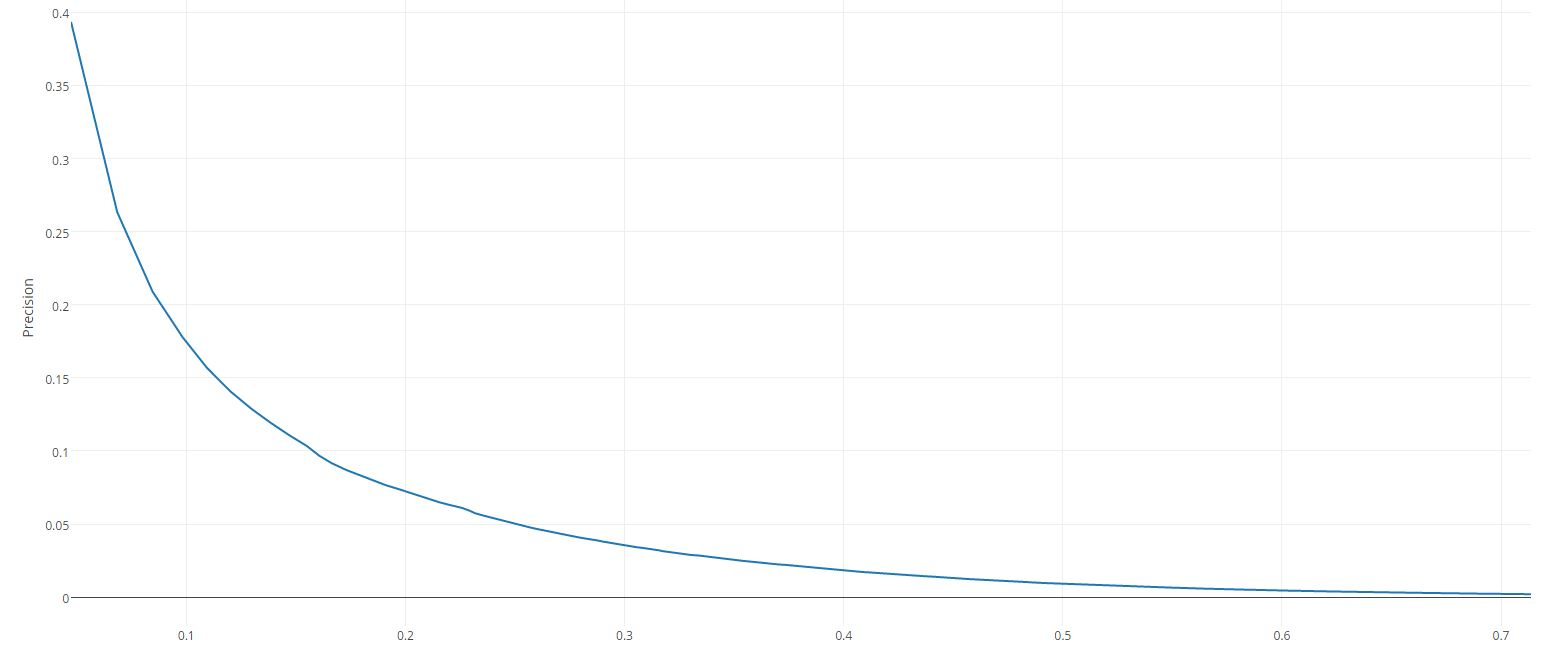
\includegraphics[width=130mm]{images/uniresult0.jpg}
	\caption{The precision-Recall chart for Unigram Language Model with smoothing 0.}
	\label{fig:uniresult0}
\end{figure}

\begin{figure}[H]
	\centering
	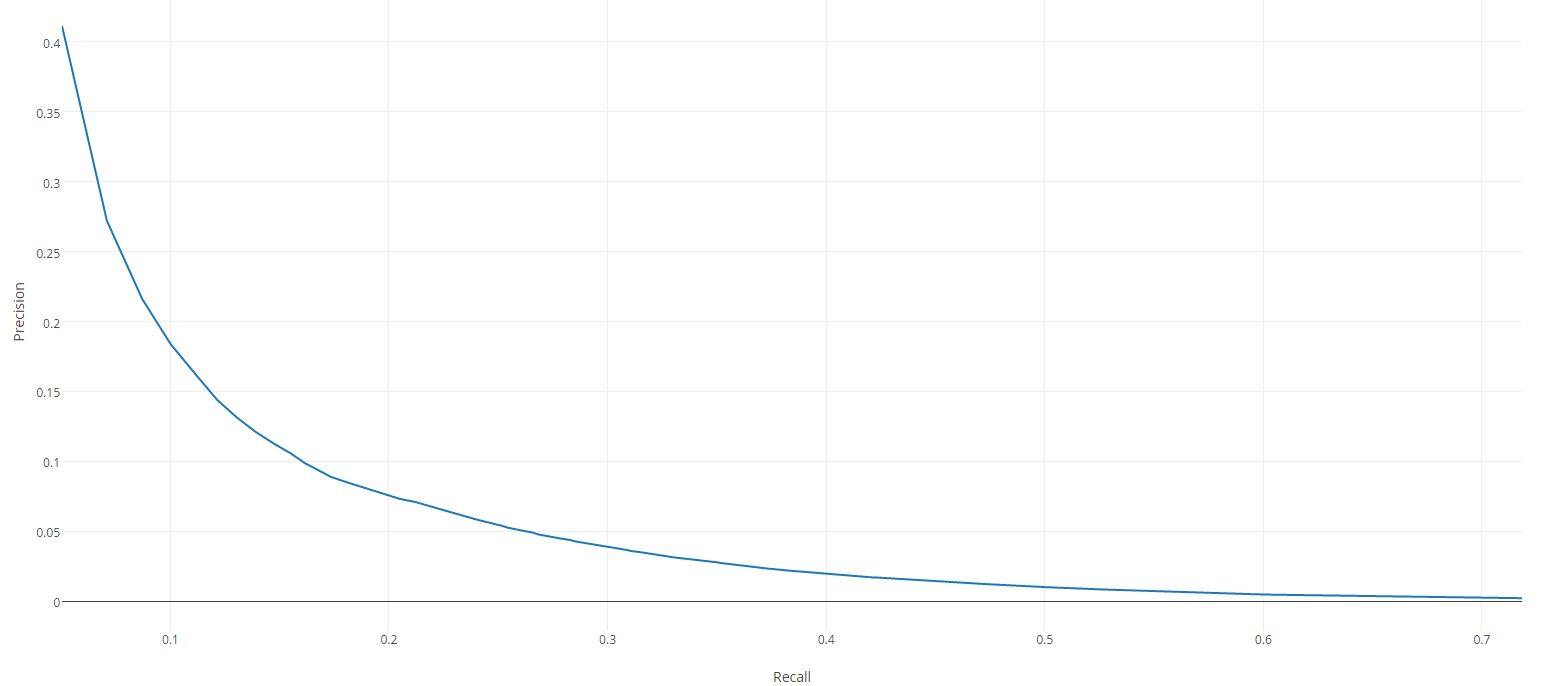
\includegraphics[width=130mm]{images/uniresult10.jpg}
	\caption{The precision-Recall chart for Unigram Language Model with smoothing 10.}
	\label{fig:uniresult10}
\end{figure}


\begin{figure}[H]
	\centering
	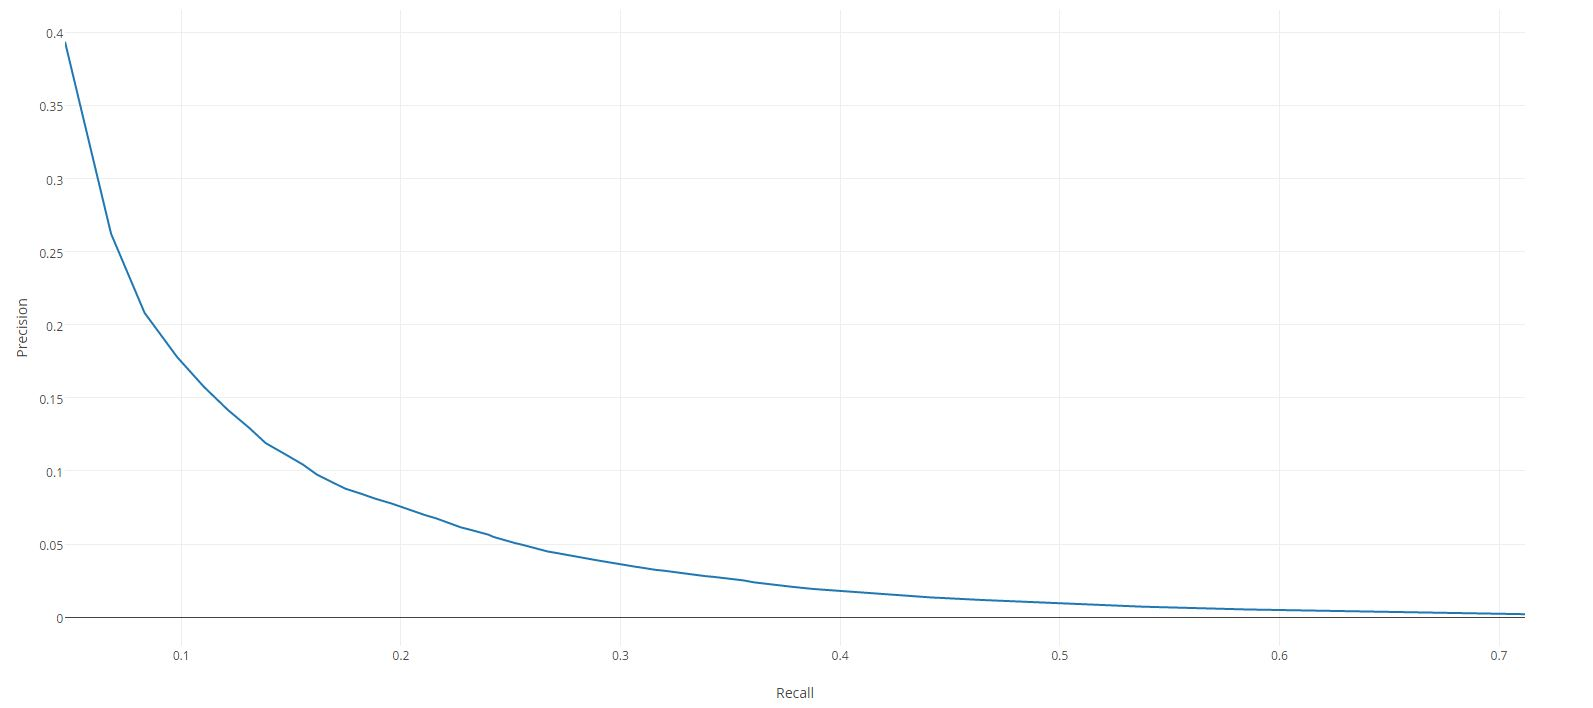
\includegraphics[width=130mm]{images/uniresult50.jpg}
	\caption{The precision-Recall chart for Unigram Language Model with cutoff 50.}
	\label{fig:uniresult50}
\end{figure}


\begin{figure}[H]
	\centering
	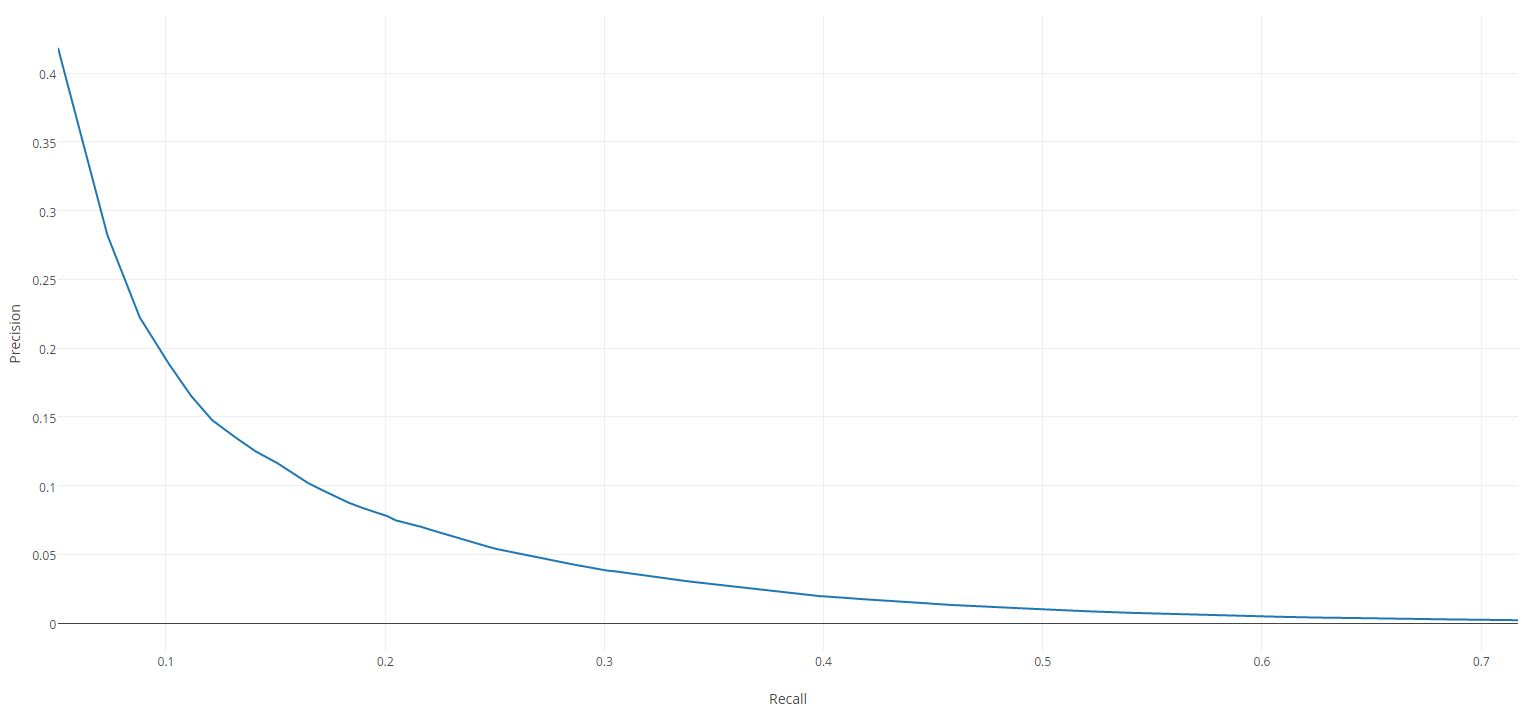
\includegraphics[width=130mm]{images/uniresult100.jpg}
	\caption{The precision-Recall chart for Unigram Language Model with cutoff 100.}
	\label{fig:uniresult100}
\end{figure}

\begin{figure}[H]
	\centering
	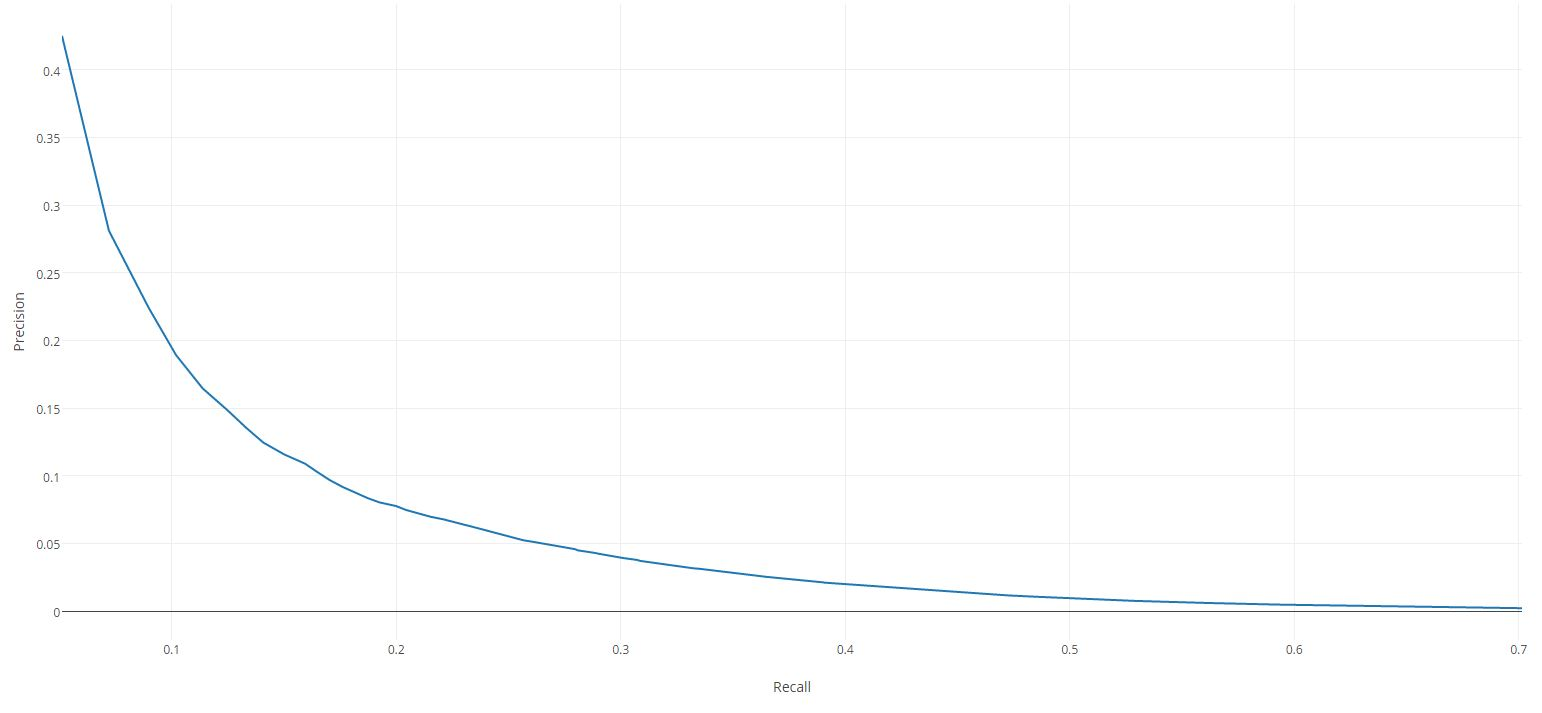
\includegraphics[width=130mm]{images/uniresult250.jpg}
	\caption{The precision-Recall chart for Unigram Language Model with cutoff 250.}
	\label{fig:uniresult250}
\end{figure}

\begin{figure}[H]
	\centering
	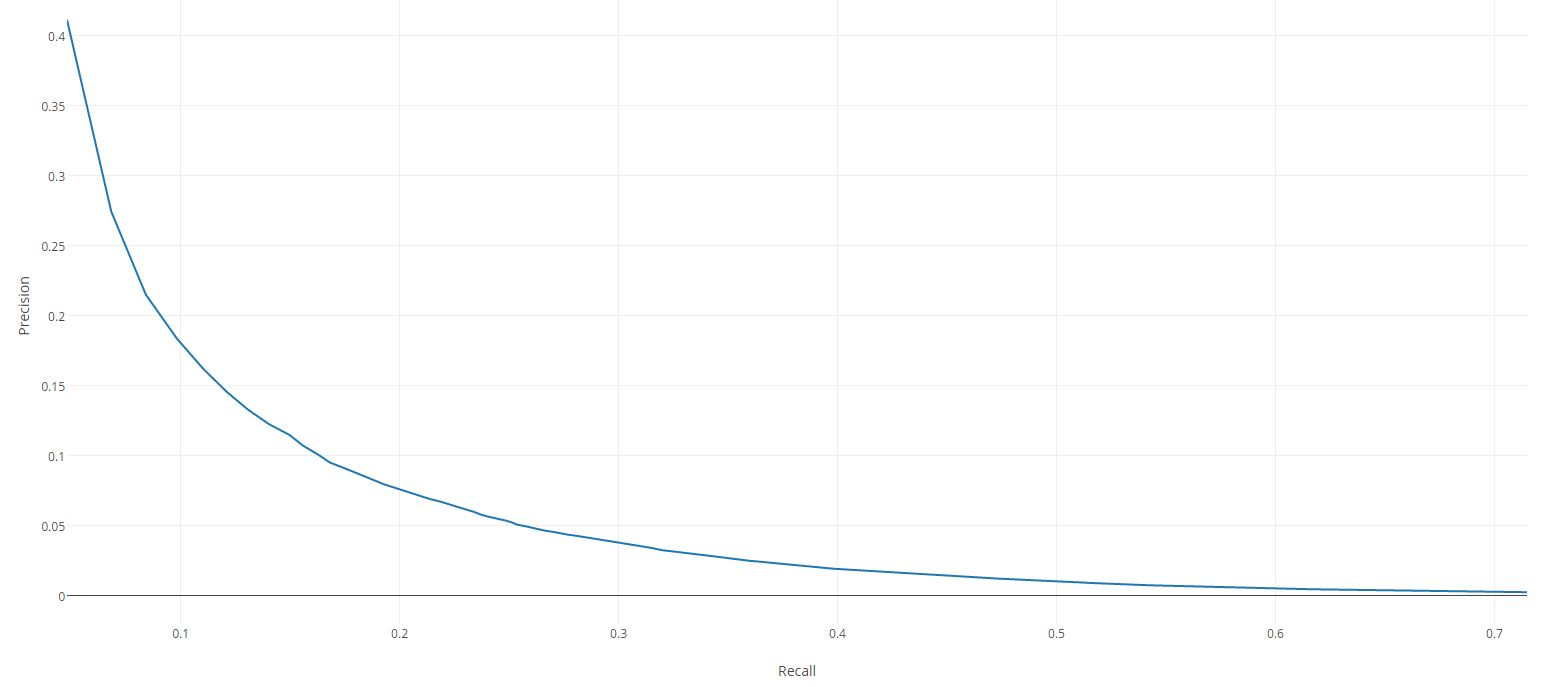
\includegraphics[width=130mm]{images/uniresult500.jpg}
	\caption{The precision-Recall chart for Unigram Language Model with cutoff 500.}
	\label{fig:uniresult500}
\end{figure}

\begin{figure}[H]
	\centering
	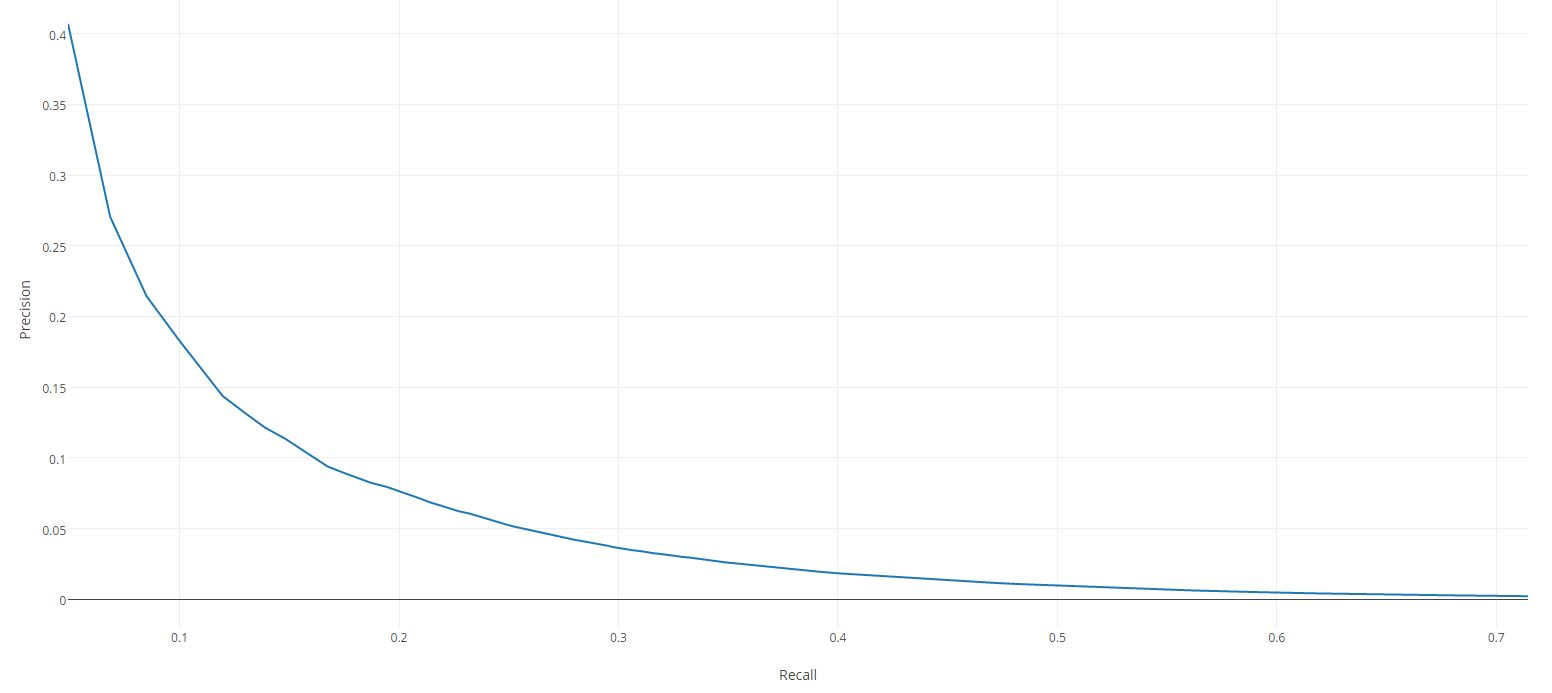
\includegraphics[width=130mm]{images/uniresult1000.jpg}
	\caption{The precision-Recall chart for Unigram Language Model with cutoff 1000.}
	\label{fig:uniresult1000}
\end{figure}



\subsubsection{Wordembedding}
\begin{figure}[H]
	\centering
	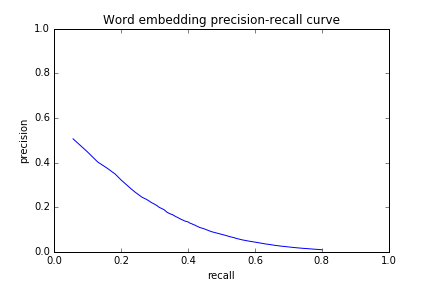
\includegraphics[width=130mm]{images/precision-recall_embedding.png}
	\caption{The precision-Recall chart for word embedding.}
	\label{fig:embeddingpresicionrecall}
\end{figure}
MAP: 0.258010537928
\begin{table}[H]
	\centering
    \begin{tabular}{| c | c | c |}
        \hline
        \textbf{\#top queries} & \textbf{Recall} & \textbf{Precision}\\ \hline
        10   & 0,2529983  & 0,2565 \\
        100  & 0,5341049  & 0,06583 \\
        250  & 0,6483118  & 0,032468  \\
        500  & 0,7281287  & 0,018326 \\
        1000 & 0,8003459  & 0,010071 \\
        \hline
    \end{tabular}
\end{table}

\subsubsection{LSI}


\subsection{Discussion}
First of all, we can see that the recall increases at we increase the number of top N queries. This is logical because the recall gives ratio between found and to-be-found. So if we would cut off at the maximum amount of documents, the recall would be 100%.
\newline
Secondly we see that the precision decreases as the amount of documents increases. 

\subsubsection{Unigram Language Model}
The simple Unigram Model is the simpelest of all methods that we attempted. It is also the fastest of all methods that we attempted. However, this speed comes at an accuracy cost.
The Simple Language Model does not account for words with a similar meaning, something the word embedding does account for and we can see that the word embedding is superior in accuracy.
[More explanation about the charts]

\subsubsection{Wordembedding}
Because the location of the word in the model gives semantic similarity, words with similar meanings are given similar vectors. This results in a more accurate result than the Unigram Language Model, as we can see in the results.
Because of the limited size of the documents, a lot of similar words are still found. If the descriptions would be longer, a more accurate result could be found and the overall accuracy would increase. But with the current length of the queries and the target collection, we think we got acceptable results.
\newline
\newline
To calculate similarity, we sum the different vectors. The main problem with this approach is that it introduces a lot of noise. Every word contains a similar value. We have already attempted to reduce this problem by removing the stopwords (which increased our results), but this is not a total solution. A more intelligent method would be using weighted sum based on other information. (e.g. using Term Frequency Inverse Document Frequency (TF-IDF) to weigh terms based on their frequency) However, we have not attempted to add TF-IDF for a weighted sum (as it would increase the computational need) and can therefore only assume that it would further increase the accuracy.

\subsubsection{LSI}



\section{Conclusion}
In retrospect to the methods, we have learned that the older models, such as the Simple Language Models performs very well while taking way less computational power. Our favorite method was Word2Vec (mostly because it gave the best results), but it takes a lot of RAM memory. In fact, the used models took up all our RAM which resulted in extra long running times because some things had to be written on the hard disk.
And finally, hyper-parameters (as used in LDA) should give better results, it was quite challenging (and fun) to analyze why the results were not as expected.
\newline
\newline
In retrospect of the assignment, we need to divide our time better, ie. prioritizing certain aspects instead of focussing on eg fine-tuning. And when using methods like Word2Vec, a cloud computer or online server can save a lot of time.
\newline
\newline
Overall, it was an interesting to work with the algorithms and see empirical results instead of just the theoretical results. We have experienced at first-hand what difficulties occur during the experiments (e.g. how important it is that all words are in a similar form).

\section{References}
\bibliographystyle{plain}
\bibliography{references}
	
\end{document}